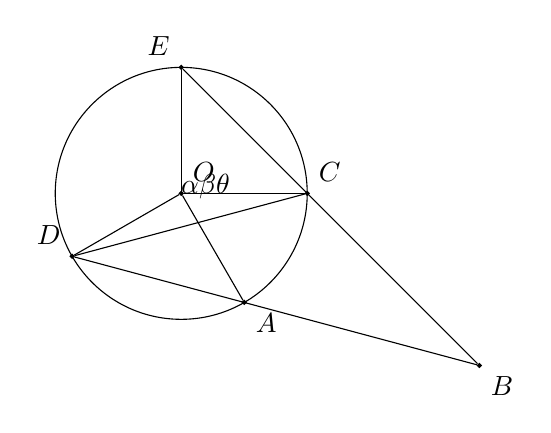
\begin{tikzpicture}
[scale=0.4,>=stealth,point/.style={draw,circle,fill = black,inner sep=0.5pt},]
%\tikzset{shift={(-3,0)}}

%innput parameters
\def\r{4}

%Labeling points
% r sin(pi/3) = 3.4641
\node (O) at (0,0)[point,label=above right:$O$] {};
\node (C) at (\r, 0 )[point,label=above right:$C$] {};
\node (A) at ({\r/2},-3.4641)[point,label=below right:$A$] {};
\node (D) at (-3.4641 , -{\r/2})[point,label=above left:$D$] {};
\node (E) at (0 , \r)[point,label=above left:$E$] {};
\node (B) at (9.4641 , -5.4641)[point,label=below right:$B$] {};


%A



%Drawing parallelogram ABCD
\draw (O) -- (A);
\draw (O) -- (C);
\draw (O) -- (E);
\draw (O) -- (D);
\draw (D) -- (B);
\draw (E) -- (B);
\draw (C) -- (D);


\draw (O) circle (\r);
%marking angles
\tkzMarkAngle[fill=orange!50,mark=](E,O,D)
\tkzMarkAngle[fill=green!50,mark=](A,O,C)
\tkzLabelAngle[pos=0.65](E,O,D){$\alpha$}
\tkzLabelAngle[pos=0.65](A,O,C){$\beta$}
%\tkzMarkAngle[fill=orange!50,mark=](E,B,D)
\tkzLabelAngle[pos=2.65](E,B,D){$\theta$}

%
\end{tikzpicture}
